\documentclass[a4paper,10pt]{report}

% Language
\usepackage[UKenglish]{babel}    % define culture for rendering (eg., hyphenation rules)
\usepackage[T1]{fontenc}       % use utf8 fonts
\usepackage[utf8]{inputenc}      % input encoding is utf8
\usepackage{lmodern}             % use font Latin Modern

% Supreme boilerplating
\usepackage{etex}                % LaTeX 2.0 features on relics
\usepackage{microtype}           % Extremely anal typographic mode
\usepackage{url}                 % Ability to create URLs
\usepackage[hidelinks]{hyperref} % Makes intradocument links, eg., contents page
\usepackage{color}               % Adds colour features. Really.
\usepackage{graphicx}            % Adds image features

% Layout
\usepackage[a4paper]{geometry}   % In case I want to set margins etc.
\usepackage{setspace}            % For setting line spacing
\usepackage{enumerate}           % Allows different types of numbering
\onehalfspacing

% Actual Packages
\usepackage{fixme}
\usepackage[authoryear, round, sort]{natbib} % References
\usepackage{amsmath}             % Imports for maths things
\usepackage{amssymb}
\usepackage{amsthm}
\usepackage{empheq}              % For highlighting mathematics
\usepackage{tikz}
\usetikzlibrary{arrows,shapes,decorations.pathreplacing,decorations.pathmorphing,calc,patterns,scopes,trees,positioning,fit}
\usepackage{pgfplots}
\pgfplotsset{compat=1.7}
\pgfkeys{/pgf/number format/relative round mode=fixed}

% Bug Fixes
\usepackage{fixltx2e}            % LaTeX bugfixes (yes really)
% "fix the natbib spacing character" - Kevin Naud�
\makeatletter
\ifdefined \NAT@spacechar
	\def\NAT@spacechar{~}
\fi
\makeatother

\hypersetup{pageanchor=false}    % Wait until actual start of writing before making page anchors


%%%%%%%%%%%%%%%%%%%%%%%%%%%%%%%%%%%%%%%%%%%%%%%%%%%%%555
% Macros

% Restarts numbering and sets format to 1, 2, 3...
\newcommand \startrealnumbers { 
	\pagenumbering{arabic}
	\setcounter{page}{1} 
	\hypersetup{pageanchor=true}
}

% Renders a bibliography on its own page, and adds a contents reference.
\def \bibliographysection {
	\cleardoublepage
	\phantomsection
	\addcontentsline{toc}{chapter}{Bibliography}
	\bibliographystyle{authordate3}
	\bibliography{bibliography}
}

\newcommand \todo \fxwarning

\begin{document}

\title{A JIT-less, Register-Mapped, Statically-Typed Virtual Machine for Interpreters}
\author{Matthew Sainsbury}
\date{\today}

% Cover Page
\begin{titlepage}

		\maketitle
	
\end{titlepage}

\pagenumbering{roman}

% Prefaces
\nakedchapter{Acknowledgements}
	To all my loyal fans

\nakedchapter{Abstract}
	\todo{align this with project proposal}
	Traditional JIT-less high-level register virtual machines simulate virtual registers in random access memory (RAM) and load virtual registers from RAM whenever they are accessed \citep{caseregistervm}. This treatise investigates an alternative approach where virtual registers are mapped to physical registers, and instructions are dispatched not only on the opcode, but also on the operands of the instruction. To emulate a virtual instruction, the interpreter jumps to the appropriate code segment in a table of implementation code based on the instruction word to be executed. This table grows in a polynomial fashion with increased virtual registers, and therefore the performance balance between table size and register pressure is investigated.

\nakedchapter{Declaration of Own Work}


\tableofcontents

\nakedchapter{Glossary}
\begin{description}
	\item[Bytecode] Program code executed by a virtual machine.
	\item[Virtual Machine] A class of programs which translate code written for one architecture to another.
\end{description}


% Main document body
\chapter{Introduction}
	\startrealnumbers
	This treatise investigates a new implementation technique for interpreted virtual machines. Two ideas are presented: register mapping between virtual machine registers and real registers, and a new dispatch method which operates on full instruction words. It is thought \todo{Weazel words?} that these two novelties might make it easier for a modern superscalar CPU to predict the behaviour of the virtual machine by reducing the amount of data dependance.
	
	This section aims to establish why such an endeavour is worthwhile by presenting a brief outline of the many existing designs for high level virtual machines.
	
	\section{Background}
		A virtual machine is a program that executes a machine code program by translating the instructions from one machine architecture to another. This allows a programmer to execute a program written for one architecture on a different architecture.
		
		A subclass of virtual machines---high-level virtual machines---are of interest in this project. A high level virtual machine runs programs for a machine which is imagined by its designer. This machine is typically more sophisticated and generic than real machines. As a consequence, a high-level virtual machine is an abstraction layer which hides the intricacies of any particular real machine. This virtual machine can be implemented for any physical architecture, resulting in the extremely useful property that code written for a virtual machine is very portable. The ``machine code'' that a high-level virtual machine executes is called its \emph{bytecode}. 
		
		The primary use for high-level virtual machines is in high-level interpreted languages, such as C$^\sharp$, Java and Python. High-level language interpreters are typically implemented with a compiler that compiles the input source code into an intermediary bytecode, which is then interpreted on a high level virtual machine. This technique is much faster than interpreting the source code line-by-line. Because the virtual machine is designed to support high-level features of interpreted languages, it is easier to write a compiler for the language targeting the virtual machine. This approach also helps to modularise the structure of the interpreter by seperating the language and context analysis structures from the host-specific implementation details \citep{structureinterpreters}.
		
		The interpretation of bytecode on any virtual machine is significantly slower than executing native code \citep{optimizingindirectbranch}. Just-in-time (JIT) compilation tries to bring ``the best of both worlds'' together. Modern JIT interpreters begin with the normal interpretation process, but while interpreting, profiles the executing bytecode to determine which parts of the bytecode would most benefit from native execution. Once it has identified these sections of bytecode, it compiles them into the host machine's instruction set and executes them natively instead of interpreting them \citep{historyjit}. Most popular virtual machines utilise JIT compilation, such as Java's JVM, and C$^\sharp$'s Common Language Runtime (CLR).
		
		Although JIT compilation is a good strategy to improve the performance of virtual machines, they have disadvantages in certain use cases. For instance, in multi-instance programs, where a program is started many times to produce many processes running the same code simultaneously. A real-world example of such a program is a web server, which spawns several identical program threads to serve web clients asynchronously. Unfortunately, multi-instance applications have become much more common as CPUs increase in core count, and stagnate in clock frequency.
		
		As shown in Figure \ref{fig:nativeprogram}, operating system kernels automatically arrange native multi-instance programs to share a read-only code space between instances \citep{sharedcodepatent}. This does not happen with an interpreted program, because the code is loaded by the interpreter, and not by the kernel itself. With an interpreter utilising a JIT compiler, each process will be doing its own tracing and JIT compilation of the bytecode, essentially compiling the same code over and over (Figure \ref{fig:interpretedprogram}). JIT compilation is a hefty procedure, so multiple compilations of the same identical code is not acceptable. Overcoming this problem require processes to have a mechanism to discover other running processes that are using the same interpreter, and then negotiate a code-sharing scheme. Implementing such a system would be very difficult. With this in mind, it is useful to explore opportunities for improvement in JIT-less interpreters so that situations where JIT compilation is inappropriate are not neglected. With this in mind, ``traditional'' high-level virtual machines will be considered. 
		
		\begin{doublefig}
			\begin{halffig}
				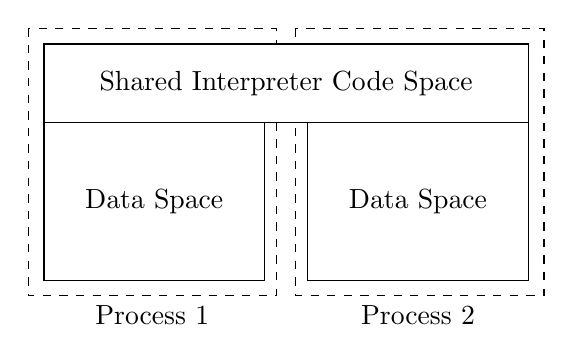
\begin{tikzpicture}
				\draw (-0.2, 0.2) [dashed] rectangle (2.95, -3.2) node[below] at (1.375, -3.2) {Process 1};
				\draw (3.2, 0.2) [dashed] rectangle (6.35, -3.2) node[below] at (4.75, -3.2) {Process 2};
				\draw (0,0) [fill=white] rectangle (6.15,-1) node[midway] {Shared Interpreter Code Space};
				\draw (0,-1) rectangle (2.8, -3) node[midway] {Data Space}; 
				\draw (3.35,-1) rectangle (6.15, -3) node[midway] {Data Space}; 
				\end{tikzpicture}
				\caption{Two native programs}
				\label{fig:nativeprogram}
			\end{halffig}
			\begin{halffig}
				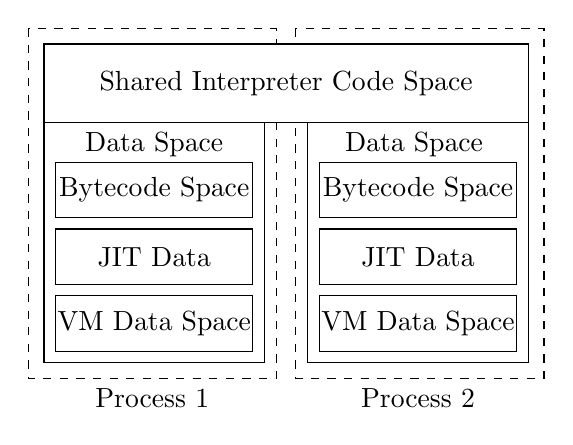
\begin{tikzpicture}
				\draw (-0.2, 0.2) [dashed] rectangle (2.95, -4.25) node[below] at (1.375, -4.25) {Process 1};
				\draw (3.2, 0.2) [dashed] rectangle (6.35, -4.25) node[below] at (4.75, -4.25) {Process 2};
				\draw (0,0) [fill=white] rectangle (6.15,-1) node[midway] {Shared Interpreter Code Space};
				\draw (0,-1) rectangle (2.8, -4.05) node[below] at (1.4,-1) {Data Space}; 
				\draw (3.35, -1) rectangle (6.15, -4.05) node[below] at (4.7,-1) {Data Space};
				\draw (0.15, -1.5) rectangle (2.65, -2.2) node[midway] {Bytecode Space};
				\draw (3.5, -1.5) rectangle (6, -2.2) node[midway] {Bytecode Space};
				\draw (0.15, -2.35) rectangle (2.65, -3.05) node[midway] {JIT Data};
				\draw (3.5, -2.35) rectangle (6, -3.05) node[midway] {JIT Data};
				\draw (0.15, -3.2) rectangle (2.65, -3.9) node[midway] {VM Data Space};
				\draw (3.5, -3.2) rectangle (6, -3.9) node[midway] {VM Data Space};
				\end{tikzpicture}
				\caption{Two interpreted programs}
				\label{fig:interpretedprogram}
			\end{halffig}
		\end{doublefig}
		
		\subsection{Traditional Virtual Machines}
			There are two general types of high-level virtual machine architectures: stack machines and register machines. 
			
			Unsurprisingly, a stack machine maintains a stack data structure where temporary values are stored, and the machine's instruction set consists mostly of operations on the stack.  \ref{fig:stackprogram} shows an example of code written for a stack machine. Notice that the operands of the instructions are implicit, and so instructions for stack machines tend to be shorter. This is the major difference between instructions for stack machines and register machines. 
		
			The bytecode of a stack machine is very simple. For each operation, a unique code (called an \emph{opcode}) is assigned. For instance, a word value~(``instruction word'') of \texttt{0x01} might represent push, while \texttt{0x02} might represent add, and so on. The introduction of literals, such as the $14$ and $8$ in the first two lines---as well as other types of additional data attached to instructions---complicates this picture, but the idea remains unchanged.
		
			A register machine contains a number of high-speed memory ``boxes'' into which temporary values are stored, called registers. Instructions generally specify which registers are involved in the operation~(``operands''). Figure \ref{fig:registerprogram} shows the same program for a register machine. In the \texttt{add} instruction, the value of \texttt{regA} is added to \texttt{regB}, and the result is stored in \texttt{regA}. This is a convention in assembly programming which will be used throughout the text.
		
			A register machine's bytecode is different, because the operands of the instruction need to be part of the instruction encoding. Typically this is implemented using bitfields. For example, consider a twelve-bit instruction word. We can reserve the first 4 bits for the opcode. This gives us a maximum of 16 opcodes. The next four bits of the instruction word can encode the first operand as an enumeration, and the same for the last four bits which can encode the second operand. If an instruction only has one operand, the last four bits are undefined. This is illustrated in Figure \ref{fig:bitfields}
			
			\begin{myfigure}
					\texttt{
						\begin{tabular}{ | l | r | r |r | }
							\hline
							Meaning & opcode & dest & src \\ 
							\hline
							add regA, regB  & 0001 & 0000 & 0001 \\
							\hline
							add regD, regC & 0001 & 0011 & 0010 \\
							\hline
							divide regB, regA & 0010 & 0001 & 0000 \\
							\hline
							print regA & 0011 & 0000 & 0000 \\
							\hline
						\end{tabular}
					}
					\caption{Register instructions using bitfields}
					\label{fig:bitfields}
			\end{myfigure}
			
			\begin{doublefig}
				\begin{halffig}
					\begin{lstlisting}
push 14
push 8
add
push 7
divide
print
					\end{lstlisting}
					\caption{Typical stack machine program}
					\label{fig:stackprogram}
				\end{halffig}
				\begin{halffig}
					\begin{lstlisting}
mov regA, 14
mov reg1, 8
add regA, regB
mov regB, 7
divide regA, regB
print regA
					\end{lstlisting}
					\caption{Typical register machine program}
					\label{fig:registerprogram}
				\end{halffig}
			\end{doublefig}
			
			\todo{Should I talk about dispatching, and virtual machine implementation in general?}
			
		\subsection{The Nature of Modern Processors}
			The landscape of processor design has changed significantly in the last thirty years. Rather than producing performance gains by arbitrarily increasing processor clock speeds, modern processor designers rely on trying to increase the per-cycle efficiency of their processors, using techniques such as instruction-level parallelism, larger and more complex cache systems, and speculative optimisation. These design issues caught the interest of academics and engineers in the 1980's \citep{modernprocessordesign}. Some of these topics will be briefly discussed in this section.
			
			\subsubsection{Instruction-Level Parallelism}
			Traditional processors executed machine instructions one at a time. Every clock cycle, an instruction would be fetched, decoded, and executed. The result of this method is that activity on a processor would move through the architecture componentwise. Only one part of the process would be ``working'' at any time---for instance, when an instruction was being decoded, the entire execution component of the processor was unused.
			
			On a processor with instruction-level parallelism, these functions can operate in parallel. An instruction can be fetched while another instruction is being decoded, and yet another instruction's operands are being fetched. A processor that can operate this way is said to have an \emph{instruction pipeline.} This results in far better utilisation of processor hardware, but introduces complexity in the processor. For instance, if one instruction writes to a memory address, and later instruction reads from the same address, the second instruction cannot complete the operand fetch stage until the first instruction has been executed. A situation where an instruction has to wait for another to complete is known as a \emph{pipeline stall,} and is a subject of much academic writing and engineering effort.
			
			\subsubsection{Cache Arrangement}
			Modern processors contain portions of high-speed memory which act as a cache to the main memory of the machine. The behaviour of this cache is an important factor for processor performance, because main memory is quite slow compared to the speed of a CPU. Modern caches are orders of magnitude larger than processors twenty years ago. 
			
			Most modern processors contain a series of specialised caches. For instance, a fourth-generation Intel Core processor has three grades or \emph{levels} of cache, and make a distinction between cache for instructions and cache for program data. Figure \ref{fig:cachenumbers} shows the arrangement of cache on such a processor. As can be seen, L1 cache is much faster, but much smaller than L2 cache. The latency in L1 instruction cache is not shown because instruction fetch is transparent to programs, but it does influence branch prediction (see later). It is advantageous for a program if most of its application data can fit in L1 data cache, and most of its code can fit in L1 instruction cache. 
			
			\begin{myfigure}
				\begin{tabular}{ | l | l | l | l | }
					\hline
					Level & Type & Size & Latency \\ 
					\hline
					\multirow{2}{*}{L1} & Instruction & 32KB & N/A \\
					& Data & 32KB & 4 cycles \\
					\hline
					L2 & Data & 256KB & 11 cycles \\
					\hline
					L3 & Data & Varies & Varies \\
					\hline
				\end{tabular}
				\caption{Cache on 4th-Gen Intel Core CPUs \citep{optimisationreference}}
				\label{fig:cachenumbers}
			\end{myfigure}
			
			\subsubsection{Branch Prediction \& Branch Target Prediction}
			Branch prediction in a process refers to the processor's ability to continue the pipelining process during a branch instruction. Ordinarily, the location of the next instruction is known to the processor---it is simply the instruction adjacent to the previous one. If the previous instruction was an instruction to branch (go somewhere else in the program), the picture becomes more complex. There are three types of branches worth mentioning:
			
			\begin{description}
				\item[Unconditional Branch:] This instruction always causes the processor to jump to the same location. The target of the branch is known as soon as the instruction is decoded.
				\item[Conditional Branch:] This branch type branches to a constant location if a condition is true. For instance, if a register is zero (``branch if zero''). The location of the next instruction is only known once the branch instruction is executed.
				\item[Indirect Branch:] A branch whose branch location is based on program data, whether in memory or in a register, or both. 
			\end{description}
			
			An unconditional branch is the easiest branch to pipeline, since the location of the next instruction is encoded in the branch instruction itself. The next instruction can be fetched as soon as the branch instruction is decoded. 
			
			A conditional branch is harder to pipeline because it is not known whether the condition is true or false before the instruction is executed, and thus what the next instruction should be. To prevent cache stalls on conditional branch instructions, modern processors implement a \emph{branch predictor}. The branch predictor will use some heuristic to predict the conditional, and load the most likely next instruction. A pipeline stall will only occur if the prediction was wrong.
			
			An indirect branch is the worst type of branch for a pipelined processor. It is very hard to predict because the branch location could depend on any data anywhere in main memory or in registers. This influence that data has on the behaviour of the program is known as \emph{data dependance} and is to be avoided whenever possible. Modern processors implement a \emph{branch target predictor} in an attempt to reduce the number of pipeline stalls. A branch target predictor is not to be confused with a branch predictor---a branch predictor predicts whether the branch will be taken, whereas a branch target predictor tries to predict where the branch will lead. A conditional branch can only lead two places---the next instruction, or the constant branch location.
			
			One common branch target predictor is a branch target buffer. A branch target buffer maintains a mapping between each indirect branch instruction, and the last target location of the branch. This strategy works well if an indirect branch always branches to the same location, but is no help if it is always different.
			
			These concepts form the background to this research, and the problems which motivate it.
	
	\section{Problem Description}
		Most physical machines are register machines. It is thought that the use of real machine registers to store the values of the virtual machine registers will help to make the operation of virtual machine programs more transparent to the physical CPU by reducing data-dependant fetches from main memory, where virtual machine registers are usually stored. Unfortunately, unlike virtual registers that are implemented in memory, real registers cannot be accessed by ``reference'' \citep{caseregistervm}. This difference complicates the implementation of a register-mapped virtual machine.
		
		Despite these difficulties, it is worthwhile to investigate designs of JIT-less register virtual machines that attempt to narrow the divide between the host and guest architecture.
	
		\todo{Do I need more?}
		
	\section{Purpose and Scope}
		The goal of this project is to investigate the feasibility of JIT-less register virtual machines for interpreters running on a modern architecture. To this end, a high-level register virtual machine will be implemented with some unique architecture features that have not been investigated or thought feasible previously.
		
		A novel dispatch process will be investigated that seeks to allow the use of physical machine registers in the implementation of virtual machine registers. To circumvent the problem of referencing real machine registers, the virtual machine will dispatch not only based on the opcode of each instruction, but on the instruction as a whole. In other words, an implementation will exist for every combination of operands in each virtual machine instruction.
	
		An instruction set architecture will be designed which will be tailored for such a dispatch method. It is anticipated that having implementations for every combination of operands in each virtual machine instruction will cause the virtual machine implementation to become very large, and so the design of the instruction set architecture will focus on keeping the number of unique instructions low.
		
		The virtual machine will target the Intel 64 host machine architecture.
		
		\subsection{Limitations}
			As the virtual machine implementation becomes very large, it will become unsuitable for operation on machines with small L1 and L2 instruction caches, because large portions of the virtual machine implementation will not remain in the instruction cache. The result is a virtual machine that is actually slower than traditional virtual machines. We will consider only modern processors with reasonably large first-level cache, for instance, the current Intel Core i7 range of processors containing 32KB of L1 instruction cache.
			
			Assuming any virtual machine register can be used as an operand for any instruction, the size of the virtual machine implementation proportional to:
			
			\[
				\sum_{o~\in~opcodes} r^n : 
					\begin{array}{l}
						n \coloneqq \text{number of operands for o} \\
						r \coloneqq \text{number of virtual machine registers}
					\end{array}
			\] 
			
			Every additional virtual machine register increases the size of the virtual machine by a polynomial factor. At some point, any performance gain received by exposing more physical registers will be negated by increasing incidence of cache misses. This is a source of a practical limitation on the number of registers in the virtual machine's architecture.
			
				
	\section{Overview of Treatise Structure}
		\todo{Will have to wait until the rest of the treatise exists for this! Tip: Design this for someone who doesn't feel like reading the whole thing. Make it easy to find specific, interesting sections.}

% 10-12 pages
\chapter{Problem Exposition}
	\section{Literature Review}
		\cite{structureinterpreters} reflect on why spending research and engineering effort on optimising interpreters is a worthwhile endeavour. Creating a host machine independent abstraction layer between original source code and machine architecture greatly simplifies writing compilers that must generate code for many platforms. This is because for every additional platform that must be supported, a separate version of the compiler targeting that platform must be developed. In a high-level language interpreter utilising a virtual machine, only the interpreter portion needs to be rewritten for different platforms, (or perhaps not even the interpreter if a high-level language is used to implement the interpreter) and the compiler remains the same. Interpreters tend to be simple compared to compilers targeting machine code, so this advantage is quite significant. Compared to native execution, interpreters also offer opportunity for more powerful usability features like debuggers, and have faster compilers, improving the write-compile-test cycle of modern software development methods.
		
		Traditionally, the high level virtual machines implemented in interpreters are stack machines. Stack machines are used over register machines for a few reasons. Instructions for stack machines are smaller, because instruction operands are implicit. This means that instruction fetching is faster. It is easier to compile code for a stack machine than a register machine because the compiler does not need to implement a register allocator \citep{caseregistervm}. However, \cite{stackregistershowdown} found that an efficient register virtual machine can execute benchmarks 32\% faster than an analogous stack machine. 
		
		\cite{caseregistervm} mentions that the first successful virtual machine interpreter ran stack-based P-code for Pascal. This was the first in a large family of stack-based bytecodes for popular languages like Smalltalk, Java and the Common Intermediate Language (CIL). This suggests that there might be historic factors involved in the prevalence of stack based virtual machines.
		
		\cite{fastjava} believes that interpreters are not well designed to suit modern architectures features like pipelining, branch prediction and caches. They also provide encouragement by saying, ``if interpreters can be made much faster, they will become suitable for a wide range of applications that currently need a JIT.''
		
		\subsection{Relevant Previous Work}
		%mark
		
		The practice of mapping virtual machine resources to host machine registers has been investigated for stack machines by \cite{stackcaching}. Ertl measured the performance of stack machines which kept the top few elements of the stack in registers. He found that direct mapping of stack positions to machine registers was only useful for the case where just the top element of the stack was cached in a register. Further caching resulted in too many load-store instructions to shuffle register values around when positions on the stack change.
		
		Ertl also attempted a technique he calls ``dynamic stack caching'' where stack elements are cached in whatever register is convenient, and an internal state machine remembers the mapping between stack positions and registers. Many versions of code to emulate each virtual machine instructions exist; the version which is executed depends on the current state of the state machine. Ertl found that this technique halves the cost of operand fetching for each additional register involved in the caching, but adds an instruction dispatch cost because of the increased number of states.
		
		In the same paper, Ertl writes the first mention of the idea of achieving register mapping between a register virtual machine and a host register machine through a table of implementations for each combination of opcode and operands, but quickly dismisses it because it would ``cause code explosion, and will probably suffer a severe performance hit on machines with small first-level caches.'' He then went on to use the R4000 MIPS processor as an example, having 8 KB of level one (L1) instruction cache.
	
		However, this approach deserves further investigation, especially with the advent of modern processors with significantly larger cache sizes---for example, 4th generation Intel Core processors, which have 32 KB of L1 instruction cache \citep{optimisationreference}, four times as much as the R4000.
	
		
	\section{Difficulties}
		Interpreters spend most of their execution time on instruction dispatch \citep{modernarchvm}. The main contributor is usually an indirect branch to the implementation code for the currently executing virtual machine instruction \citep{optimizingindirectbranch}. Every interpreter has at least one indirect branch in dispatch code \citep{modernarchvm}. Because these indirect branches are in the instruction dispatch portion of the interpreter, they are executed for every virtual machine instruction. This closely couples interpreter speed to efficiency of branching.
		
		Modern architectures tend to have long pipelines and perform branch target prediction to load the target of an upcoming branch before the branch instruction is executed. Branch target misprediction is very expensive in these architectures, because the execution of a branch happens late in the pipeline but affects the start of the pipeline \citep{optimizingindirectbranch}. Traditional interpreter designs that were optimal on older architectures perform poorly on modern pipelined architectures because branch prediction accuracy is a big factor on performance on these architectures. These interpreter designs hide the logic governing branching patterns from the branch predictor. \cite{yeti} explains this by saying ``the control transfer from one body to the next is data dependent on the sequence of instructions making up the virtual program.'' This is an atypical scenario for modern processors, and they are not designed optimally for this task.
		
		To be more concrete, a popular method to predict indirect branch targets is a branch prediction buffer (BTB). BTB makes the assumption that the targets of indirect branches are unlikely to change \citep{yeti}, and maintains a table of the last target of each branch instruction. When the branch is encountered again, BTB predicts the target will remain the same. However, this is not the case for interpreter dispatch, because the indirect branch is based on the current virtual machine opcode, which could be any one of the instructions in the virtual machine instruction set. For each of these opcodes, the interpreter will branch to a particular section of code to emulate the virtual machine instruction. In other words, the BTB prediction will be accurate only if the opcode being dispatched is the same as the previous dispatch. Because it is not very likely that the virtual machine will see many of the same opcode over and over, the BTB fails to predict the branch target most of the time. Opcodes ``fight'' for the single target record in the BTB that corresponds with the indirect branch in the dispatch code.
		
		\cite{structureinterpreters} found that the branch misprediction penalty consumes up to half of the execution time on some interpreters. This high proportion is a result of the fact that most of an interpreter's time is spent in the instruction dispatch process.
		
		One way to get around this problem is by duplicating the indirect branch instruction, resulting in a separate BTB entry for each branch instruction \citep{fastjava}. This can be done by duplicating the dispatch code at the end of each virtual instruction implementation, instead of jumping back to a common dispatch code. In contrast, the traditional focus in branch optimisation was to make the code path as short as possible.
		
% 10-12 pages
\chapter{Solution Design}
	When designing the virtual machine architecture, it will be beneficial to remember this succinct heuristic by \cite{structureinterpreters}: ``Well-designed VMs are tailored for both easy compilation from the source language and fast interpretation on real machines.''\todo{too fluffy?}
	\todo{Biggest factor for performance is the design, so we spent a lot of time on it}

\chapter{Evaluation Methods and Results}

% Last chapter
\chapter{Conclusion}
	
	\section{Opportunities for Future Development}
	
	\section{Reflection}

% Bibliography
\bibliographysection

\end{document}